\chapter{Pyramid of Moore}

\vspace{\baselineskip}

\begin{paracol}{2}

\begin{boss}{Gargoyles}
    \varwb
    \begin{round}{1}
        \faris \rightCommand{\gilToss}
        \cara \leftCommand{\gilToss}
        \bartz \rightCommand{\gilToss}
        \faris \rightCommand{\gilToss}
    \end{round}
    \varwe
\end{boss}

\begin{menu}{After Gargoyles}
    \varwb
    \begin{itemMenu}
        \hiPotionMenu \ally{People missing 100+ HP}
    \end{itemMenu}
    \begin{abilityMenu}
        \faris \ability{!\black}
    \end{abilityMenu}
    \begin{jobMenu}
        \cara Ninja \textbf{(\pointLeft)(\pointDown)(\pointLeft) \ability{!\white}}
        \bartz Thief \textbf{(2\pointRight)} \ability{!\combine} \optimize
        \begin{itemize}
            \item[] \equip{\stealthRobe, \greenBeret}
        \end{itemize}
    \end{jobMenu}
    \varwe
\end{menu}

\switchcolumnTwice[*]
\begin{encounter}{Aspis}
    \varwb
    \begin{round}{1}
        \bartz \rightCommand{\combine} \then \battleGroup{\hiPotion \space + \phoenixDown} \textit{(RESURRECTION)} \then \enemy{Aspis} 
    \end{round}
    \varwe
\end{encounter}

\begin{enumerate}[resume]
    \item Stop and wait for the spikes to come out to get poisoned
\end{enumerate}

\switchcolumn
\vspace{-2cm}
\begin{misc}{If You Get a MachinHead}
    \begin{notes}
        \item \miscHl{Need to get Lamia's Kiss off before he gets a turn}
    \end{notes}
    \begin{round}{1}
        \bartz \rightCommand{\combine} \then \battleGroup{\maidensKiss \space + \eyedrop} \textit{(LAMIA'S KISS)} \then \enemy{MachinHead}
        \cara \leftCommand{\throw} \then \thunderScroll 
        \faris \leftCommand{\throw} \then \thunderScroll 
    \end{round}
    \begin{round}{2}
        \bartz \rightCommand{\combine} \then \battleGroup{\eyedrop \space + \revivify} \textit{(ELEMENTAL EDGE)} \then \enemy{MachinHead}
        \cara \leftCommand{\throw} \then \thunderScroll 
        \faris \leftCommand{\throw} \then \thunderScroll 
    \end{round}
\end{misc}

\switchcolumn
\begin{menu}{After Opening the Sarcophagus}
    \varwb
    \begin{jobMenu}
        \bartz Knight \textbf{(A)} \ability{!\black} \optimize
    \end{jobMenu}
    \begin{itemMenu}
        \hiPotionMenu \ally{Bartz}
    \end{itemMenu}
    \varwe
\end{menu}

\begin{boss}{Mummy x3}
    \varwb
    \begin{round}{1}
        \cara \leftCommand{\throw} \then \flameScroll
        \faris \leftCommand{\throw} \then \flameScroll
        \bartz \rightCommand{\black} \then \fire
    \end{round}
    \varwe
\end{boss}

\begin{menu}{After Mummies}
    \varwb
    \begin{jobMenu}
        \faris Mediator \textbf{(\pointUp)}
        \cara Thief \textbf{(2\pointRight)} \ability{!\escape}
    \end{jobMenu}
    \varwe
\end{menu}

\switchcolumnTwice[*]
\begin{enumerate}[resume]
    \item \battleGroup{Escape is the right command}
    \item Don't use the 2nd switch before the chest room
    \item Use the left switch to get the chests
    \item Grab the \pickup{9000 Gil} and \pickup{8000 Gil} chests on the right
\end{enumerate}

\switchcolumn
\begin{misc}{Shifting Floor Room}
    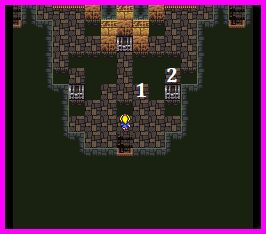
\includegraphics[scale=0.449]{../Graphics/Steps/177. Pyramid 2.jpeg}
    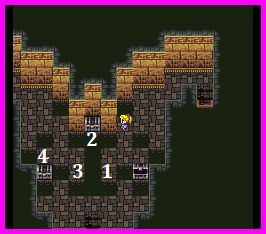
\includegraphics[scale=0.449]{../Graphics/Steps/178. Pyramid 3.jpeg}
\end{misc}

\switchcolumn
\resume
\begin{enumerate}[resume]
    \item Grab the \pickup{Gold Hairpin} chest on the right in the shifting floor room
    \item Take the right exit
    \item Grab the left chest containing \pickup{12000 Gil}
    \item Head back upstairs
    \item On the way out, grab the \pickup{Guard Ring} and \pickup{Ribbon}
\end{enumerate}

\end{paracol}